%!TEX root = ../report.tex
\chapter{Architecture}
\label{cha:architecture}

To create a system for automatic creation of a sentiment lexicon, two different approaches have been developed based on the graph propagation approach and the \ac{pmi} approach, outlined in Section~\ref{sec:automatic_generation_of_sentiment_lexica}. In addition, a lexicon based classifier has been developed, utilizing the features of the lexicon created. In this chapter the three systems are described individually in addition to two core system components: tweet preprocessor and vocabulary tokenization, used in all three systems. After initial tests of the two lexicon creation approaches, the \ac{pmi} approach outperformed the graph propagation approach and became our main focus of the two. This is specifically reflected in a more sophisticated $n$-gram creation process. 


\section{Tweet Preprocessor} 
\label{sec:tweet_preprocessor}
Our system implements preprocessing as a set of simple functions, each taking in a string, performing a simple operation, and returning the resulting string. This simple design allows chaining several preprocessors one after another achieving complex results, while remaining easily reusable because of the simplicity of each single preprocessor. Additionally, we implement two ways of chaining the preprocessors: by text or by word. A set of preprocessors chained together by text will perform the filter operation on the entire text, while preprocessors chained together by word will perform the operation at word level and will ignore words marked as "protected".\footnote{In our implementation a word is marked as protected if it begins and ends with "||".} This is particularly important with emoticons, as we often want to remove non-alphanumeric signs from the text, and most emoticons contain non-alphanumerical signs. With this approach we can first identify all the emoticons, mark them as "protected", and then apply the remove non-alphanumerical signs preprocessor at word level. This will remove all non-alphanumerical signs except the ones that are part of an emoticon. \\

\begin{figure}[t]
    \centering
    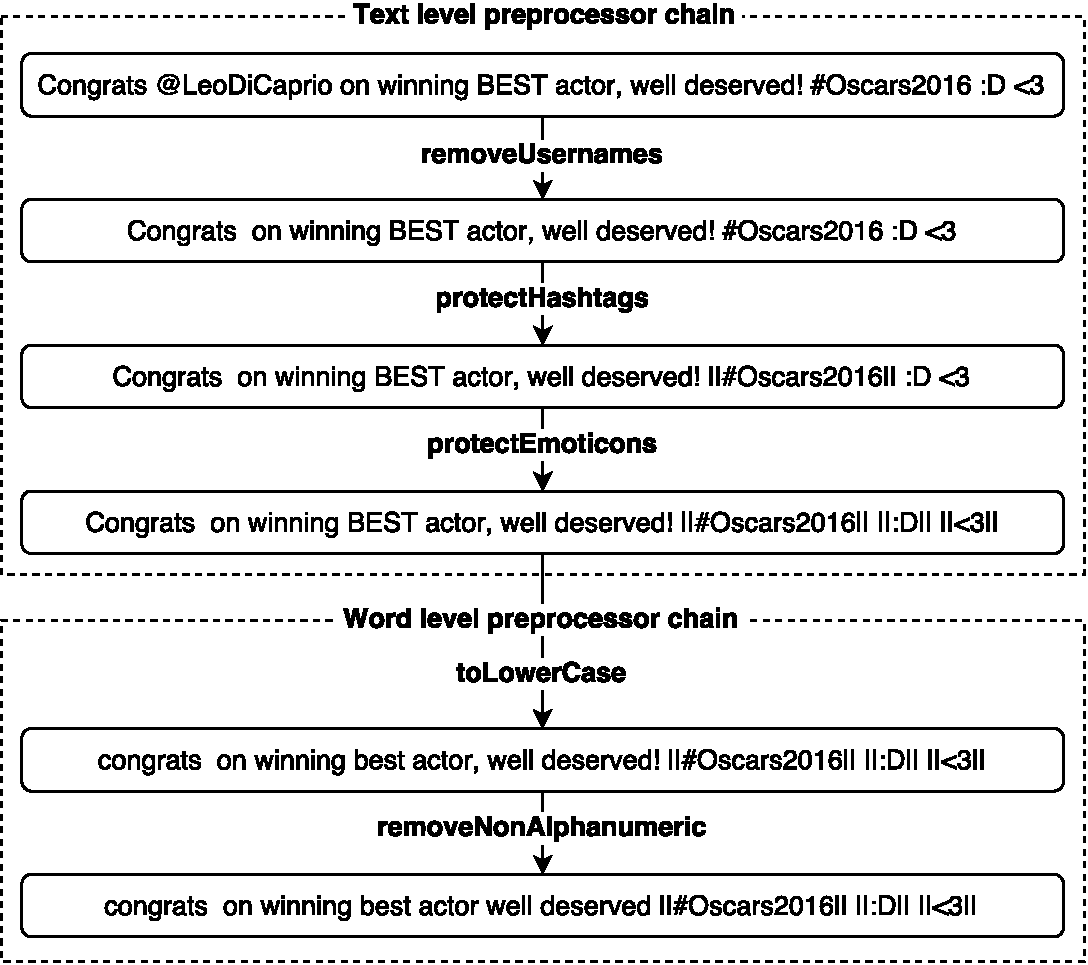
\includegraphics[width=\textwidth]{./figs/chain_preprocessor}
    \caption{Effect of different preprocessors on a tweet}
    \label{fig:chain_preprocessor}
\end{figure}

Figure~\ref{fig:chain_preprocessor} illustrates a series of text-level and word-level preprocessors chained one after another. Notice how hashtags are still intact and upper-cased after the $removeNonAlphaNumeric$ and $toLowerCase$ preprocessors because they were marked as "protected" and therefore ignored. \\

\begin{table}[t]
    \setlength\tabcolsep{2pt}
    \begin{tabular}{| l | p{8.3cm} |}
        \hline
        \textbf{Filter} & \textbf{Description} \\ \hline
        %HTMLUnencode
        normalizeForm & Normalizes letters to Latin alphabet if possible, for example "Déjà vu" becomes "Deja vu" \\ \hline
        unicodeEmojisToAlias & Translates Unicode emoji characters to their alias as given by emoji-java library \\ \hline
        removeUnicodeEmojis & Removes all Unicode emoji characters \\ \hline
        protectEmoticons & Marks all ASCII emoticons as "protected" \\ \hline
        removeEmoticons & Removes all ASCII emoticons \\ \hline
        removeUsername & Removes all username mentions \\ \hline
        removeEMail & Removes all e-mail addresses \\ \hline
        removeHashtag & Removes all hashtags \\ \hline
        protectHashtag & Marks hashtags as "protected" \\ \hline
        removeRTTag & Removes RT tags \\ \hline
        removeURL & Removes URLs \\ \hline
        %removeApostrophes & Removes characters often found mid word, such as '
        removeNonSyntact & Removes all non alphabetic or punctuation characters \\ \hline
        removeNonAlphanum & Removes all non alphanumerical characters \\ \hline
        %removeFreeDigits & Removes 
        toLowerCase & Transforms all letters to lower case \\ \hline
    \end{tabular}
    \caption{List of preprocessors used in our system}
    \label{tab:master_filters}
\end{table}

\subsection*{Elongation Correction}
\begin{figure}[t]
    \fbox{\parbox{\textwidth}{
    \begin{enumerate}
        \item For every word in the vocabulary, extract the condensed form, where sequences of a repeated letter are replaced with a single instance of that letter.\\
        E.g., \textit{niiiice → nice, realllly → realy, ...}
        \item Create sets of words sharing the same condensed form.\\
        E.g., \{\textit{nice, niiice, niccccceee, ...}\}, \{\textit{realy, really, realllly, ...}\}
        \item Remove sets which contain 5 or less unique variations.\\
        E.g., \{\textit{committee, committe, commitee}\}
        \item From each set, remove words with distribution less than 5\% among the words that are condensed to the same form.\\
        E.g., \{\textit{god: 15\%, good: 80\%, goood: 2\%, godd: 1\%, goood: 1\%, gooood: 1\%, ...}\} → \{\textit{god: 15\%, good: 80\%}\}
    \end{enumerate}}}
    \caption{Steps in the creation of a condensed form dictionary}
    \label{fig:canonical_dict}
\end{figure}

To handle elongation, described in Section~\ref{sec:text_filtering}, a correction process utilizing the Levenshtein distance algorithm (Section~\ref{sec:levenshtein}) and the condensed form of words, is applied to all words. The process consists of two parts: a four step dictionary creation part inspired by \cite{brody11}, shown in Figure~\ref{fig:canonical_dict}, and a word correction part using the created dictionary. In order to correct a word, the word is first reduced to its condensed form, before being looked up in the dictionary. If found, the dictionary returns the most likely spellings of the initial word. Then the Levenshtein distance is calculated between the initial word and each of the returned words, before correcting the initial word to the closest match. This way, with a dictionary containing both "good" and "god", the word "goddd" is 2 removals away from "god" or 2 removals and 1 addition from "good", and will therefore be reduced to "god".

\section{Vocabulary Tokenization}
\label{sec:tokenization}
In both our lexicon based classifier and our \ac{pmi} lexicon approach the process of tokenization is used. The process consists of splitting sentences into what we call "optimal" tokens, which are the longest non-overlapping $n$-grams also found in a given vocabulary. The $n$-grams that were not found in the provided vocabulary are tokenized as unigrams. The vocabularies used should contain the most relevant $n$-grams within the given context. The longest $n$-grams are preferred based on the assumption that the longer $n$-grams provide more precise information than the shorter $n$-grams. \cite{Goodman01abit} argues that there is little to gain with $n$-grams longer than $n=5$, stating that the performance, in terms of perplexity and entropy of the language model, plateaus between $n$-grams of length 5-7. \citeauthor{Goodman01abit} further states that building a model based on $n$-grams of lengths up to $n=5$ appears to give a good tradeoff between computational resources, in terms of runtime and memory usage, and performance.  \\

\begin{figure}[t]
    \centering
    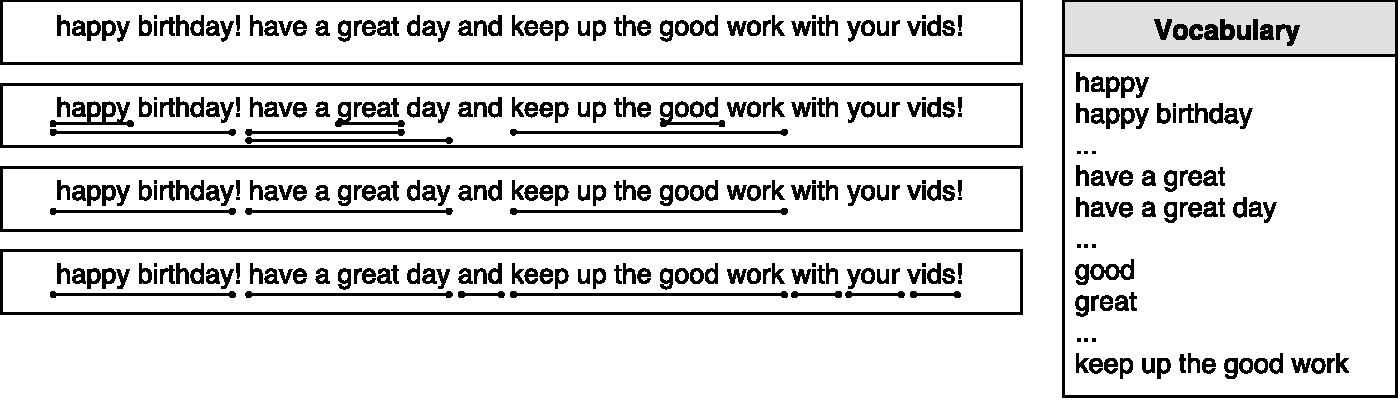
\includegraphics[width=\textwidth]{./figs/tweet_tokenization}
    \caption{The tokenization process shown step by step}
    \label{fig:tweet_tokenization}
\end{figure}

Figure~\ref{fig:tweet_tokenization} illustrates the process of vocabulary tokenization of a tweet. The different stages of tokenization of a tweet are shown on the left, while the relevant phrases in the vocabulary are shown on the right. The first stage of vocabulary tokenization is to find all $n$-grams in the tweet that are also present in the vocabulary. Then, we select the longest $n$-gram found and remove all the $n$-grams that overlap with it. The final stage is to tokenize the remaining words in the tweet as unigrams. The reason for keeping the words not present in the vocabulary is that these words may be intensifiers or negators, which are excluded from our lexicon. Additionally, keeping these words is important for negation, since it affects the $x$ next words.

\section{Tweet Streaming API Dataset}
\label{sec:twitter_streaming_dataset}
\subsection*{Raw Tweets}

\begin{figure}[t]
    \centering
    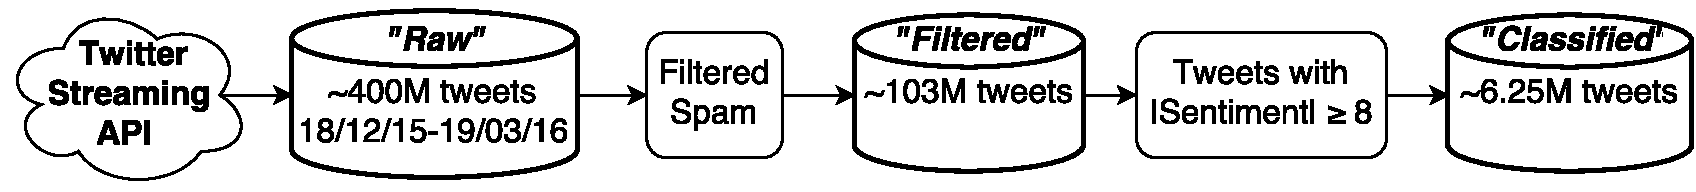
\includegraphics[width=\textwidth]{./figs/twitter_datasets}
    \caption{Datasets created using Twitter Streaming API}
    \label{fig:twitter_steaming_api_datasets}
\end{figure}


To be able to create a sentiment lexicon based on raw tweets, a large corpus of tweets was needed. We downloaded about 400 million tweets using the Twitter Streaming API.\footnote{\url{https://dev.twitter.com/streaming/reference/post/statuses/filter}} The tweets were gathered in the period 18/12/2015-19/03/2016 (92 days), with about 4 million tweets downloaded each day.

\subsection*{Filtered Dataset}
\label{sec:filtered}
After that, we filtered the entire raw tweets dataset, removing all tweets considered to be noise. A tweet was considered to be noise if:

\begin{itemize}
    \item Contained "RT @"
    \begin{itemize}
        \item Nearly half of all downloaded tweets were retweets, most of the retweets are of few original tweets, failing to remove these would make some phrases over-represented.
    \end{itemize}
    \item Contained a URL
    \begin{itemize}
        \item Tweets containing a URL were usually response to, opinion of or simply the first ~100 characters of a news story. These tweets are generally unhelpful to analyze without also analyzing the contents of page linked to itself. 
    \end{itemize}
    \item Contained $^{\circ}$ symbol
    \begin{itemize}
        \item There is a surprising amount of automated weather and GPS services connected to Twitter that regularly tweet current weather or location, this simple rule excludes most of them.
    \end{itemize}
    \item Ended with a number
    \begin{itemize}
        \item Spammers often tweet the same message over and over with an incrementing number attached to the end of the tweet, this is probably to combat Twitter's own automatic spam detection.
    \end{itemize}
\end{itemize}

The resulting dataset contained about 103 million tweets and is used to generate the $n$-grams.\\

\subsection*{Labeled Dataset}
\label{sec:labeled}
To be able to use the \ac{pmi} approach when creating a sentiment lexicon, a large dataset of labeled documents --- or in our case labeled tweets --- was needed. For the approach to produce good and reliable results, the amount of labeled tweets we needed was much higher than the manually annotated tweets made available through \ac{semeval}, which in turn meant that we needed a method for labeling tweets ourselves. \\

The approach we came up with was to label tweets using our lexicon based sentiment analysis system, described in Section~\ref{sec:lexicon_based_sentiment_analysis_system} with the manually annotated sentiment lexicon \textit{AFINN} by \cite{AFINN}. For the labeling to be as accurate as possible, only tweets with absolute sentiment score above a certain value were labeled and extracted. The value chosen was found using grid search and is a trade-off between precision and recall. Low values will give higher recall as we will be able to classify more tweets, but it will also lower precision. \\

Based on the \textit{Filtered} dataset, with 103 million unlabeled tweets, the labeling process yielded a labeled dataset containing 6.25 million tweets, of which 58.7\% were labeled as positive and the remainder as negative.


\section{Automatic Lexicon Creation}
In order to achieve the goal of automatic creation of a sentiment lexicon, two different approaches, both identified during our literature review presented in Section~\ref{sec:automatic_generation_of_sentiment_lexica}, have been developed. The developed approaches are based on the graph propagation lexicon described in Section~\ref{sec:graph_propagation_algorithm} and the \ac{pmi} lexicon described in Section~\ref{sec:pointwise_mutual_information}. 


\subsection{Graph Propagation Lexicon}
\label{sec:graph_propagation_lexicon}
Our implementation of the graph propagation approach consists of four steps. A vocabulary identification step, a context-vector creation step, a graph creation step and finally a sentiment propagation step.   


\subsection*{Vocabulary Identification}
During the vocabulary identification step a set of candidate $n$-grams are identified and selected, forming a context vocabulary. Each tweet is processed into all possible $n$-grams with length up to $n=5$, where candidate $n$-grams are selected based on their occurrence frequency in the large unlabeled \textit{Filtered} dataset. All $n$-grams below a frequency threshold, in addition to all $n$-grams ending on one of the stopwords in Table~\ref{tab:master_stopwords} or containing one of the intensifiers in Table~\ref{tab:intensifiers} are filtered out. Infrequent $n$-grams are filtered out, because the context vector to be created in the subsequent step is too unreliable on infrequent $n$-grams. In contrast to \cite{MohammadKZ2013}, where all $n$-grams containing stopwords are removed, we only remove $n$-grams ending on a stopword. This is because we believe that the ending stopword does not provide the $n$-gram with any additional information, but $n$-grams starting with or containing a stopword may change the $n$-grams sentiment or reverse it completely. For example, \textit{"the best"} is more positive than just \textit{"best"}, and the phrase \textit{"the shit"}, which is a positive phrase, is captured in addition to the word \textit{"shit"}, which on its own is negative. $N$-grams containing intensifiers were removed due to the fact that the automatic lexicon creator was developed in parallel to our lexicon based classifier. The classifier namely detects and uses intensifiers in the classification process as described in detail in Section~\ref{sec:lexicon_based_sentiment_analysis_system}. The resulting context vocabulary forms a collection of all candidate entries for the sentiment lexicon to be created in the following steps.  


\subsection*{Context Vector Creation}
\label{sec:context_vector}
To be able to compare the candidate $n$-grams against each other, a context vector is created for all of them. This is achieved by following the COALS method presented by \cite{Rohde06animproved}. The context vector of an $n$-gram is created by summing up the word frequencies of the $x$ number of words occurring to the left and $x$ number of words to the right of the $n$-gram over all mentions of the $n$-gram in the dataset. For the context vectors, representing the context of the $n$-gram, to be as accurate as possible, the context vector word frequencies are weighted according to the distance away from the $n$-gram. This is done using a ramped window of size 6. A word appearing right next to the $n$-gram on either side will increase the frequency of that word in the context vector by 6 for that side, while a word appearing six words away will increase the frequency by 1 for that side, as shown in Figure~\ref{fig:ramped_window}. 

After all initial context vectors have been created, a matrix containing all $n$-grams is created. In the matrix each row contains the context vectors of all selected $n$-grams and each column contains the occurrence frequency of a single word occurring in the different vectors. When the matrix has been initialized, the values are normalized using Pearson Correlation as described in Section~\ref{sec:pearson_correlation}. Finally, all negative values are set to 0, while all positive values are squared, resulting in our final context vectors. \\

\begin{figure}[t]
    \centering
    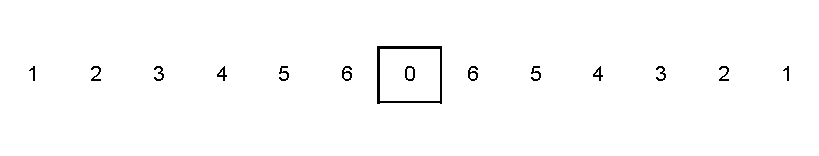
\includegraphics[width=\textwidth]{./figs/ramped_window}
    \caption[Ramped window of size 6]{Ramped window of size 6. The square represents an occurrence of an $n$-gram in a sentence. The numbers on either side represents the weights of the surrounding words.}
    \label{fig:ramped_window}
\end{figure}


\subsection*{Graph Creation}
When all candidate entries have been selected and their respective context vectors have been calculated, the graph is created. The graph consists of nodes, representing the candidate entries, and edges with weights, representing the similarity between the nodes. In order to create the edges, the similarity between all pairs of $n$-grams, represented by their context vectors, is calculated using the cosine similarity measure as described in Section~\ref{sec:cosine_similarity}. Following the approach suggested by \cite{Velikovich2010}, an edge is created between two nodes if their cosine similarity is greater then a predefined threshold. The edge weights of the created edges are set to the calculated cosine similarity. 

\subsection*{Sentiment Propagation}
Using the Graph Propagation algorithm outlined in Section~\ref{sec:graph_propagation_algorithm}, the seed nodes propagate their sentiment values through the finished graph. In our implementation, each seed node can affect nodes that are connected to it via two or less other nodes. When all seed nodes have propagated their sentiment value, the final sentiment value of each node is calculated by subtracting the sum of all negative max paths from the sum of all positive max paths. The negative and positive max paths to a node, are the maximum sentiment values each connected seed node affects the node with. A node with more paths to positive than negative seed nodes, will most likely get a positive sentiment value. Nodes with few paths to seed nodes, or an approximately equal number of paths to both positive and negative seed nodes are likely to get a sentiment value close to zero. Finally, the lexicon is created by extracting all the $n$-grams and their sentiment values. 

\subsection{PMI Lexicon}
\label{sec:pmi_lexicon_creation}
Similarly to our implementation of the Graph Propagation approach, our \ac{pmi} lexicon approach is divided into a series of steps consisting of vocabulary identification, counting vocabulary occurrences in a polarized dataset and sentiment calculation, as illustrated in Figure~\ref{fig:creator_overview}.
\begin{figure}[t]
    \centering
    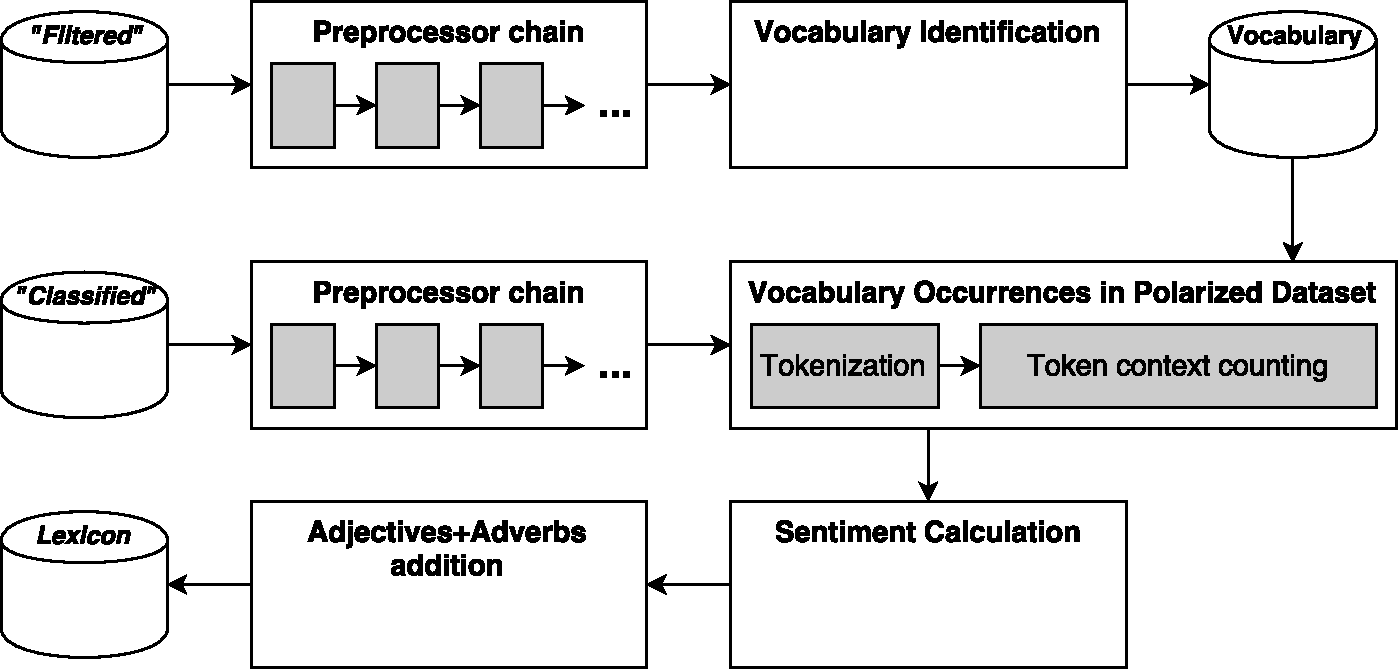
\includegraphics[width=\textwidth]{./figs/creator_overview}
    \caption{Architecture of the PMI lexicon creation system}
    \label{fig:creator_overview}
\end{figure}

\subsection*{Vocabulary Identification}
Similarly to the vocabulary identification step in Section~\ref{sec:graph_propagation_lexicon}, the \ac{pmi} lexicon vocabulary identification step also extracts and selects candidate $n$-grams for a context vocabulary based on the large unlabeled \textit{Filtered} dataset. However, the process of selection is quite different. Whereas the selection process in our graph propagation approach is strictly based on $n$-gram frequency, the selection process in our \ac{pmi} lexicon implementation uses the \ac{pmi} $n$-grams, method described in Section~\ref{sec:pointwise_mutual_information}. For an $n$-gram with $n>1$ to be selected, the \ac{pmi} of the included words needs to be higher than a predefined threshold. This way only $n$-grams containing words that together mean something or form a common phrase are selected. In addition, $n$-grams ending on a stopword or containing intensifiers are filtered out the same way as described in Section~\ref{sec:graph_propagation_lexicon}. Unigrams are not selected as candidate entries for the context vocabulary in this process, but are introduced to the system in the following two steps. \\

\begin{figure}[t]
    \centering
    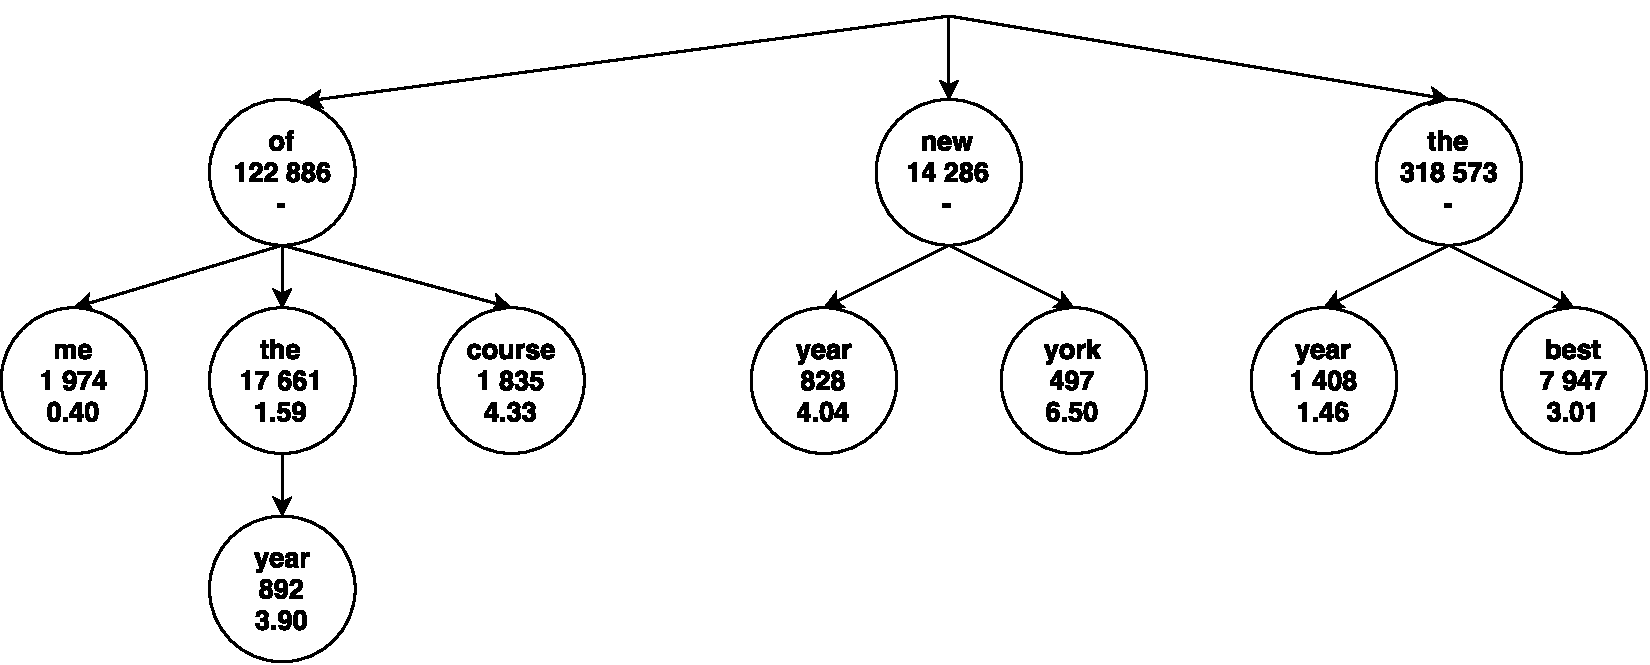
\includegraphics[width=\textwidth]{./figs/token_trie}
    \caption{Segment of a $n$-gram trie}
    \label{fig:trie}
\end{figure}

Figure~\ref{fig:trie} illustrates the process of identifying the vocabulary. Our implementation uses the trie data structure to count the number of occurrences of $n$-grams. The second line in each node is the number of times the $n$-gram has occurred in the dataset, while the third line is the $n$-gram's \ac{pmi} value. The $n$-gram "of me" is more frequent than "of course", but "of course" has much higher \ac{pmi} value. By setting two thresholds, one for frequency and one for \ac{pmi}, we can extract only the meaningful $n$-grams.

\subsection*{Vocabulary Occurrences in Polarized Dataset}
In order to calculate sentiment values of $n$-grams in our context vocabulary, the \textit{Labeled} dataset is used. For each entry in the dataset the tokenization process, described in Section~\ref{sec:tokenization}, is applied, splitting the entries into "optimal" tokens. The "optimal" tokens are the longest possible non-overlapping $n$-grams found in the context vocabulary created in the previous step. Each individual token holds counters for occurrences in positive and negative contexts. The positive context counter for a token is incremented by 1 for each time the token appears in an entry labeled as positive and the same applies for the negative context counter for tokens appearing in negative entries. The counting process utilizes the same trie data structure used when identifying the vocabulary in the previous step.


\subsection*{Sentiment Calculation}
For each $n$-gram in the context vocabulary, a sentiment value is calculated. This is achieved by using the number of times each $n$-gram occurs in positive tweets and in negative tweets found in the previous step and apply Equation~\ref{eq:sentiment_score_final} as described in Section~\ref{sec:pointwise_mutual_information}. $N$-grams occurring more frequently in negative tweets than in positive will get a negative score, while $n$-grams occurring more frequently in positive tweets will get a positive score. $N$-grams occurring just as frequent in positive tweets as in negative tweets will get a score close to zero. Finally, the lexicon is created by adding all $n$-grams with absolute sentiment value above a defined sentiment value threshold and an occurrence frequency in the \textit{Labeled} dataset above a set frequency.

\subsection*{Adjective and Adverb Addition}
With the created lexicon from the previous step, all unigrams are run through an adjective and adverb addition algorithm, adding all missing adjective and adverb forms of the unigram to increase the coverage of the lexicon. The missing adverbs and adjective forms are derived based on a set of rules\footnote{Forming Comparative and Superlative Adjectives:\\ \url{http://www.eflnet.com/tutorials/adjcompsup.php} \\and Forming Adverbs from Adjectives:\\ \url{http://www.edufind.com/english-grammar/forming-adverbs-adjectives/}} and are added to the lexicon only if they were previously encountered in the above tokenization process. The newly added adverbs and adjectives are assigned the same sentiment value as their related $n$-gram, based on the assumption that most adverbs and adjective forms of an adjective convey approximately the same sentiment. The resulting lexicon forms the final \ac{pmi} lexicon.

\section{Lexicon Based Sentiment Analysis system}
\label{sec:lexicon_based_sentiment_analysis_system}
The lexicon based Sentiment Analysis system accepts single tweets or a set of tweets and outputs a predicted classification per tweet. The predicted classification is determined by running each tweet through three main stages: preprocessing, analysis and classification, as shown in Figure~\ref{fig:classifier_overview}.

\begin{figure}[t]
    \centering
    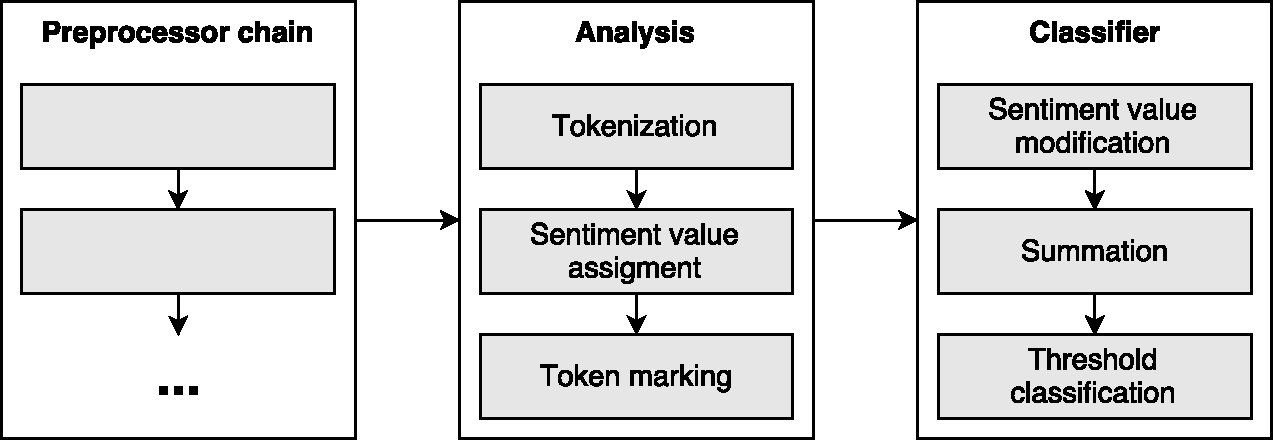
\includegraphics[width=\textwidth]{./figs/classifier_overview}
    \caption{Architecture of the lexicon classifier system}
    \label{fig:classifier_overview}
\end{figure}

\subsection*{Analysis}
After a tweet has been preprocessed, as described in Section~\ref{sec:tweet_preprocessor}, the resulting preprocessed tweet is analysed. The analysis consists of detecting negation cues, intensifier words as well as the use of punctuation marks such as: "!" and "?", and assigning sentiment values. This is done by first applying the tokenization process (Section~\ref{sec:tokenization}), splitting the preprocessed tweet into optimal tokens using the provided sentiment lexicon as vocabulary. Then the optimal tokens are looked up in the provided sentiment lexicon and assigned the lexicon value given its existence. Tokens are then marked, that is, each token is checked against a list of negation cues and intensifier words. If a token matches one of the negation ques, the following $x$ tokens are marked as negated. If a token matches an intensifier word, the next token is marked as intensified. Finally, a sentence ending in "!" or "?" will mark all the tokens in the sentence as intensified.


\subsection*{Classification}
Based on the information retrieved in the analysis step, the tweet is classified. The tokens are traversed and a classification value is calculated as a sum of the sentiment values of the individual tokens. The individual token's sentiment value depends on three variables: lexicon sentiment value of the token, whether or not the token was marked as in a negated context, and whether or not the token was marked as being intensified. If a token does not exist in the lexicon, its sentiment value is zero. The sentiment value of each token found in the lexicon is calculated as follows:

\begin{equation}
    Token Sentiment Value(token) = (L \cdot I) - N
    \label{eq:token_sentiment}
\end{equation}
where $L$ is the lexicon value of the token, $I$ is the intensification value of the token and $N$ is the negation value. When a token is not intensified $I=1$. When a token is not negated $N=0$. \\

The value of $I$ for a token is dependent on what intensifier word or punctuation mark it is affected by. Some intensifier words such as \textit{"kind of"} or \textit{"hardly"} will work as a dampeners with $I$-values between 0 and 1. Words like \textit{"incredibly"} or \textit{"extremely"} will on the other hand work as boosters with $I$-values above 1. A token can be intensified by both an intensifier and a punctuation mark. In such case, $I$ is the product of the intensification constant of the intensifier and the intensification constant of the punctuation mark. The $I$-values of "!" and "?" and the $N$ value along with their influence ranges are determined through the grid search. \\

The final sentiment score of a tweet is then calculated based on the sentiment values of the tokens:

\begin{equation}
    Tweet Sentiment Value = \sum\limits_{i=1}^{n} Token Sentiment Value(n)
\end{equation}

Finally, a tweet is classified as either positive, negative or neutral by comparing the $TweetSentimentValue$ against two thresholds, if the value is lower than $LowerNeutralThreshold$, the tweet is classified as negative, if the value is higher than $HigherNeutralThreshold$, the tweet is classified as positive, otherwise the tweet is classified as neutral. The thresholds are also determined through the grid search.

\glsresetall

